\documentclass[fleqn,12pt]{project}

\setlength{\columnsep}{0.55cm}
\setlength{\fboxrule}{0.75pt}

\definecolor{color1}{RGB}{0,0,90}
\definecolor{color2}{RGB}{0,20,20}

\usepackage{tcolorbox,listings}
\lstset{
	showstringspaces=false,
  tabsize=2,
  breaklines=true,
  columns=fullflexible
}
\tcbuselibrary{breakable}

\usepackage{hyperref}
\hypersetup{hidelinks,colorlinks,breaklinks=true,urlcolor=color2,citecolor=color1,linkcolor=color1,bookmarksopen=false,pdftitle={Title},pdfauthor={Author}}

\JournalInfo{

\includegraphics[width=2.5cm]{Figures/engineering-logo}
\Archive{}
}

\PaperTitle{ENR 280 Design Project Report (Fall 2022)}

\Authors{AJ Garcia, Ph.D.\textsuperscript{1}*.}
\affiliation{\textsuperscript{1}\textit{School of Engineering, 
  University of Mary, Bismarck, North Dakota}}
\affiliation{*ajgarcia@umary.edu}


\Keywords{}
\newcommand{\keywordname}{Keywords}

\Abstract{
  This is a \LaTeX template you can use to write up your design project report for ENR 280. The purpose for the design report for this project is to put together a document that outlines the background, theory, ideas, methodology of the design process, designs, proposed manufacturing techniques, prototypes, management, and analysis for the remote control car and various structures students will design and prototype. The objective of this design project is to practically apply the material students learn in their technical engineering courses and to experience the process of designing and managing an engineering project.   
\
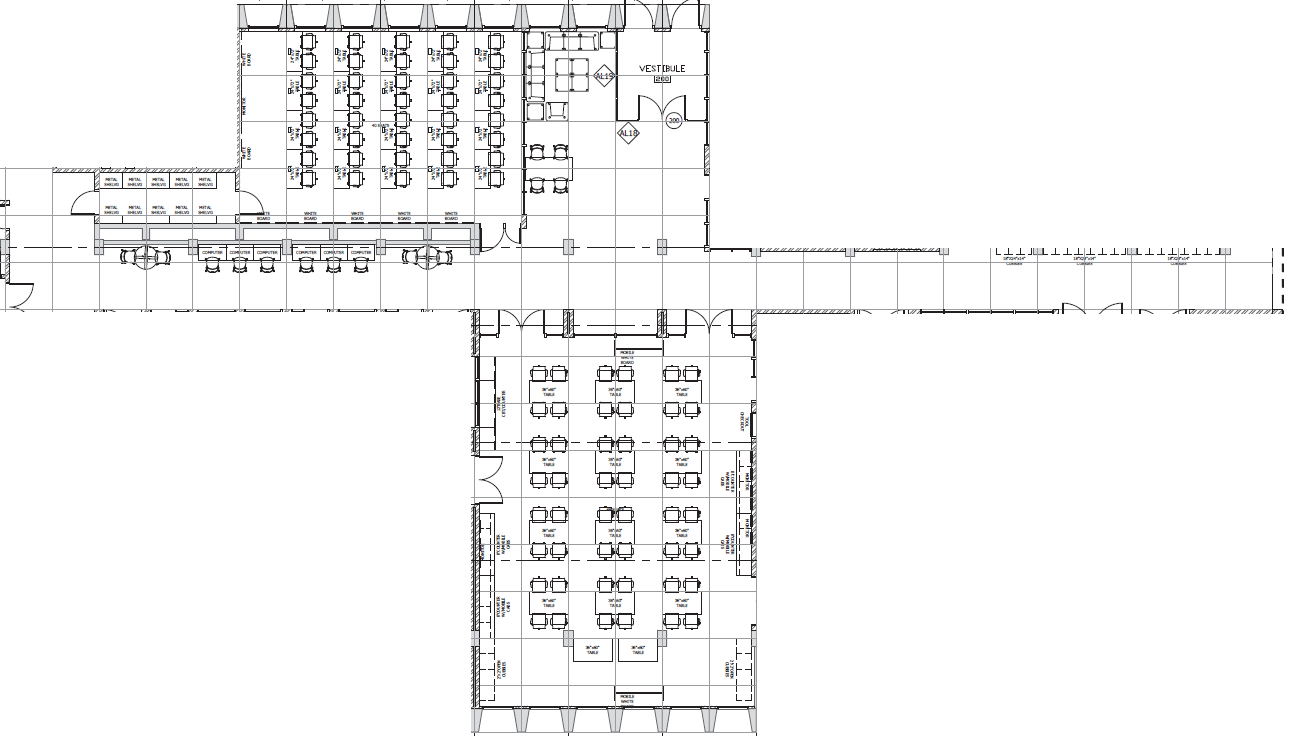
\includegraphics[width=17cm]{Figures/Floorplan}
}

\begin{document}

\flushbottom
\maketitle
\newpage
\tableofcontents
\thispagestyle{empty}
\newpage
\section*{Executive Summary}
\addcontentsline{toc}{section}{Executive Summary}

\newpage
\section{Design Problem and Objectives}

This is the design project assignment for the course ENR 280 Engineering Design Lab 1. The project assigned to each group is to design a remote control car and parts of the race track, which includes designing both a dynamic and static structure. The race course will be constructed in the University of Mary Engineering Building and occupy the Senior Design Center, Engineering Fundamentals classroom, and the Engineering building hallway and lobby depicted in Figure \ref{fig:Fig1} . In this course, ENR 280 students are tasked to present and document designs and prototypes that would be ready for manufacturing, which will take place in the sequent class, ENR 281 - Engineering Design Lab 2. Course deliverables include a detailed project report, prototypes of designs, and a presentation. 

\begin{figure}\centering
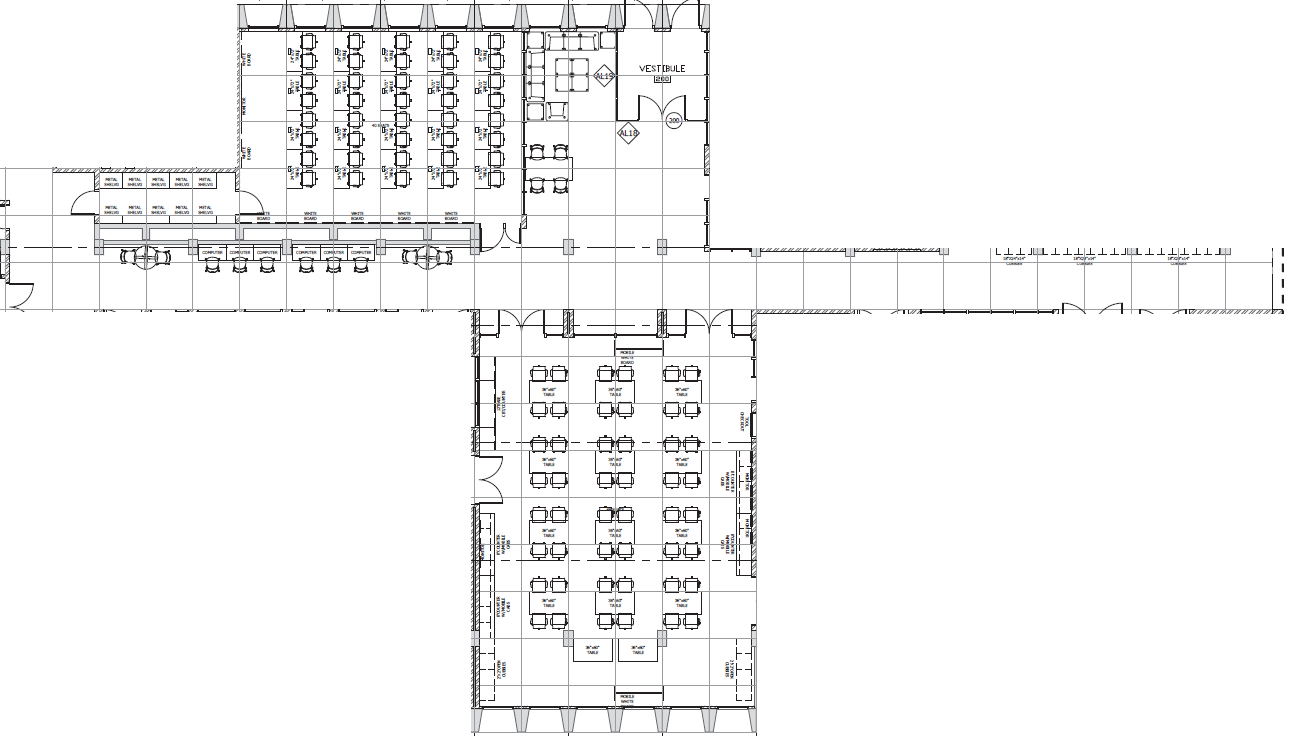
\includegraphics[width=17cm]{Figures/Floorplan}
\caption{Engineering Building Space for the Marauder's Cart course}
\label{fig:Fig1}
\end{figure}
\subsection{Design Specifications}

Each of these designs had to satisfy the requirements set out by the professor. A breakdown of the specifications required of your teams design items are stated in Table \ref{table:Table1} .

\begin{table}
\caption{Design Specifications}
\begin{center}
\small
\begin{tabular}{|cl|}
\hline
\bf{Need}\phantom{11000000000}&
\begin{tabular}{|p{5.5cm}|p{7cm}}
\bf{Design} & \bf{Specifications} \\
\end{tabular}\\
\hline
\end{tabular}
\begin{tabular}{|cl|}
\hline
Car \phantom{110000000000} &
\begin{tabular}{|p{5.5cm}|p{7cm}}
Arduino remote controlled car & Wireless mounted video camera for driver view  \\
 & No weapons/hacking/signal jamming    \\
 \end{tabular}\\
\hline
\end{tabular}
\begin{tabular}{|cl|}
\hline
Dynamic Structure &
\begin{tabular}{|p{5.5cm}|p{7cm}}
 Bridge & Span: At least 12 feet, no piers (single span)    \\
  & Width Capacity: At least 3 cars    \\
  & Maximum Deflection: $<$L/200 with all cars   \\
& Arduino controlled   \\
 & Activation: Sensors    \\
  & Type: TBD    \\
  & Movement: TBD    \\
 \end{tabular}\\
\hline
\end{tabular}
\begin{tabular}{|cl|}
\hline
Static Structure \phantom{N0}&
\begin{tabular}{|p{5.5cm}|p{7cm}}
 Jump Ramp  &  \\
 \end{tabular}\\
\hline
\end{tabular}
\end{center}
\label{table:Table1}
\end{table}


\subsection{Project Objectives}
The purpose and prime objective of the design project is for us to experience the entire design process and the putting together a document that outlines the background, theory, ideas, methodology of the design process,
designs, proposed manufacturing techniques, prototypes, management, and analysis for the remote control car and various structures
students will design and prototype. The objective of this design project is to practically apply the material students learn in their
technical engineering courses and from their own independent research, and to experience the process of designing and managing an engineering project.

%%%%%%%%%%%%%%%%%%%%%%%%%%%%%%%%%%%%%%%%%%%%%%%%%%%%%%%%%%%%%%%%%%%%%%%%%%%%%%%%%%%%%%%%%%%%%%%%%%%%
\newpage
\section{Literature Review}

Introduce the areas that will be covered in the literature review and why. Focus on the theory and background of the topics you are discussing, present what the a reader looking to duplicate your work would really need to know before trying to understand your design work.

\subsection{Jump Ramps}
For example, in order to be able to design a Jump Ramp one has to have a good understanding of how to calculate projectiles. So you'll want to present a basic explanation of the concept of what a jump ramp is and \textbf{relevant equations so the reader now has enough understanding to interpret your design work.} 
So for a understanding a projectile, one needs to know that the only acceleration that the body experiences during it's flight is gravity. This allows us to use simplified kinematic equations in a two dimensional space as all accelerations are known and are constants. Equations \ref{eq:y} and \ref{eq:x} below are  kinematic equations that describe the position of a projectile in the x and y directions with respect to time.

\begin{equation}
	y = y_0 + (v_0)_yt + \frac{1}{2}a_yt^2
\label{eq:y}
\end{equation}
\begin{equation}
	x = x_0 + (x_0)_xt
\label{eq:x}
\end{equation}
\begin{itemize}
\item x or y is final position in it's respective direction.
\item $x_0$ or $y_0$ is the initial position in it's respective direction.
\item $(v_0)_x$ or $(v_0)_y$ is the initial velocity in it's respective direction.
\item $a_y$ is the Acceleration in the y direction (this is gravity, the only acceleration the projectile experiences).
\end{itemize}


In addition to these equations, equations derived from energy and momentum principles provide us ways to solve the projectiles without the variable of time or position, respectively. These are shown etc...
\subsection{Bridges}

Do the same thing for bridges (or your static sturcture) here. Discuss the general information on bridges \textbf{as well as relevant theory/equations} in order to comprehend your design work. For example, in order to be able to design the bridge to satisfy the design specifications set out, one must have a basic understanding of what deflection is and how to calculate it. Here you'll want to present a basic theoretical description of what deflection is and an equation on how it can be determined. For example, for a point load, equation \ref{eq:delta}  can be used to determine the deflection at the point where the point load is applied on a beam. 

\begin{equation}
	\delta = \frac{Pa^2(L-a)^2}{3EIL} \\
\label{eq:delta}
\end{equation}

\begin{itemize}
\item $\delta$ is deflection
\item P is the point load
\item E is modulus of Elasticity
\item I is area moment of inertia
\item L is span length
\item a is the a dimension in the Point Load image shown in Figure \ref{fig:Fig2}.
\end{itemize}

Equations like this are derived and readily available for standard load cases such as point loads and distributed loads acting on a beam, as shown in Figure \ref{fig:Fig2}.
\begin{figure}\centering
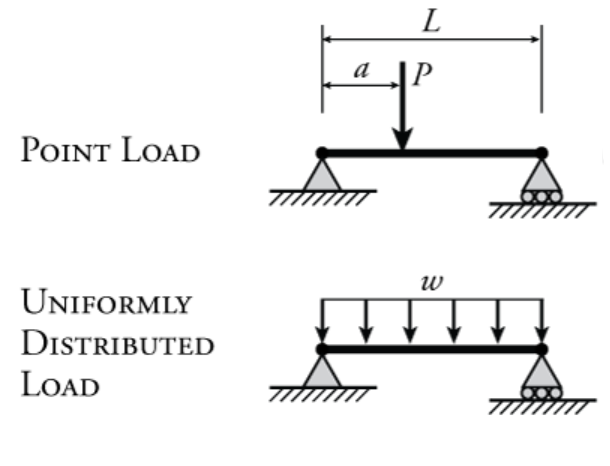
\includegraphics[width=6cm]{Figures/Loads}
\caption{Point and Distributed Loads on a Beam \cite{bib:Mechanics}}
\label{fig:Fig2}
\end{figure}

\subsection{Cars}

Discuss relevent background and theory on car frames, chassis, wheels \textbf{steering}, etc...

\subsection{Arduino Controls}
Discuss the required control logic for both the remote control car and dynamic structure. Explain any significant calculations or algorithms performed. Present the final codes with commentary as shown below.

\begin{tcolorbox}[breakable, title=\textbf{fade.h}]
\lstinputlisting[language=C++, basicstyle=\scriptsize]{Code/fade.h}
\end{tcolorbox}

Code above from \cite{bib:Fade}

%%%%%%%%%%%%%%%%%%%%%%%%%%%%%%%%%%%%%%%%%%%%%%%%%%%%%%%%%%%%%%%%%%%%%%%%%%%%%%%%%%%%%%%%%%%%%%%%%%%%
\newpage
\section{Design Conceptualization, Initial Ideas, Process and Decisions}

\subsection{Design Concepts and Initial Ideas}
\subsubsection{Jump Ramp}
\subsubsection{Bridge}
\subsubsection{Car}

\subsection{Process and Decisions}
\subsubsection{Jump Ramp}
\subsubsection{Bridge}
\subsubsection{Car}

%%%%%%%%%%%%%%%%%%%%%%%%%%%%%%%%%%%%%%%%%%%%%%%%%%%%%%%%%%%%%%%%%%%%%%%%%%%%%%%%%%%%%%%%%%%%%%%%%%%%%%%%%%%%%%
\newpage
\section{Detailed Design}
\subsection{Jump Ramp}
\subsubsection{Assumptions}
\subsubsection{Functions and Meeting Specifications}
\subsubsection{Prototypes}
\subsubsection{Manufacturing}
\subsubsection{Final Design}

\subsection{Bridge}
\subsubsection{Assumptions}
\subsubsection{Functions and Meeting Specifications}
\subsubsection{Prototypes}
\subsubsection{Manufacturing}
\subsubsection{Final Design}

\subsection{Car}
\subsubsection{Assumptions}
\subsubsection{Functions and Meeting Specifications}
\subsubsection{Prototypes}
\subsubsection{Manufacturing}
\subsubsection{Final Design}

\newpage
\section{Work Breakdown Structure}

\section{Scheduling}

\section{Bill of Materials}

\section{Conclusions}


\newpage
\bibliography{references}{}
\newpage
\section*{Appendix}
\addcontentsline{toc}{section}{Appendix}

This is where you'll want to attach your code, computer calculations, hand calculations etc...

You want to include the summarized final results or samples of data within the report itself, but the bulk of your calculations should be here. Anything within the report should be typed, including sample calculations.

Include final (and relevant sample) drawings or figures within the report as it pertains to the text. Only include drawings and/or figures in the appendix if it's supplemental to the text. 
\end{document}
